\documentclass[twoside,11pt,letter]{article}

\usepackage{times}
\usepackage{latexsym}
\usepackage{graphicx}
\documentclass[12pt,letter]{article}
\usepackage[letter, portrait, left=1in, top=1in, right=1in, bottom=1in]{geometry}
\usepackage[english]{babel}
\usepackage[utf8]{inputenc}
\usepackage{algorithm}
\usepackage[noend]{algpseudocode}
\usepackage{amsmath}
\usepackage{mathtools}
\usepackage{fancyhdr}
\usepackage{amssymb}
\usepackage{graphicx}
\usepackage{tikz-qtree}
\usepackage{tikz}
\usepackage{blindtext}
\usepackage{chngcntr}
\pagestyle{fancy}
\DeclarePairedDelimiter\abs{\lvert}{\rvert}%
\DeclarePairedDelimiter\norm{\lVert}{\rVert}%
\usepackage{url}
\usepackage[utf8]{inputenc}

\usepackage{listings}
\usepackage{xcolor}

%for code
\lstdefinestyle{mystyle}{
  backgroundcolor=\color{backcolour},   commentstyle=\color{codegreen},
  keywordstyle=\color{magenta},
  numberstyle=\tiny\color{codegray},
  stringstyle=\color{codepurple},
  basicstyle=\ttfamily\footnotesize,
  breakatwhitespace=false,         
  breaklines=true,                 
  captionpos=b,                    
  keepspaces=true,                 
  numbers=left,                    
  numbersep=5pt,                  
  showspaces=false,                
  showstringspaces=false,
  showtabs=false,                  
  tabsize=2
}

%New colors defined below
\definecolor{codegreen}{rgb}{0,0.6,0}
\definecolor{codegray}{rgb}{0.5,0.5,0.5}
\definecolor{codepurple}{rgb}{0.58,0,0.82}
\definecolor{backcolour}{rgb}{0.95,0.95,0.92}

%\aclfinalcopy % Uncomment this line for the final submission
%\def\aclpaperid{***} %  Enter the acl Paper ID here

%\setlength\titlebox{5cm}
% You can expand the titlebox if you need extra space
% to show all the authors. Please do not make the titlebox
% smaller than 5cm (the original size); we will check this
% in the camera-ready version and ask you to change it back.
\newcommand\BibTeX{B\textsc{ib}\TeX}
\title{\textbf{Wearable SONAR for the Blind}}
\author{\normalsize
  Tarun Thathvik\\
  \normalsize
  \texttt{thathvik@nyu.edu}
  \and
  \normalsize
  Smrithi Thudi\\
  \normalsize
  \texttt{srt381@nyu.edu}
  \and
  \normalsize
  Vedant Desai\\
  \normalsize
  \texttt{vbd223@nyu.edu}
}
%   Second Author \\
%   Affiliation / Address line 1 \\
%   Affiliation / Address line 2 \\
%   Affiliation / Address line 3 \\
%   \texttt{email@domain} \\


\date{}
\begin{document}
\maketitle
\begin{abstract}
In the spirit of helping the blind with a wearable device was built around the functionality and to potentially replace a traditional cane. This device vibrated based on the feedback from the SONAR to perceive the distance of the objects in the surrounding. Several calibration features were incorporated for user convenience. This device runs on an 8-core Parallax Propeller micro-controller.
\end{abstract}


\section{Inspiration}
Hugh Herr, a famous American rock climber who has shattered the limitations of his disabilities, is a strong believer of the philosophy that technology could help disabled persons to live a normal life. In one of his TED talks, Herr said “Humans are not disabled. A person can never be broken. Our built environment, our technologies, is broken and disabled. We the people need not accept our limitations, but can transfer disability through technological innovation”. These were not just words but the ideology he lived by; today he uses Prosthetic legs and claims to live a normal life. So yes, technology can not only improve the quality of human life but also neutralize human disability; and we aim to tackle the visual impairment with simple SONAR technology and a controlled vibration to perception. This could potentially replace a cane.

\section{Research and Survey}
In order to make a device that will be very accessible to the blind, information gathered during a survey done by Vedant Desai in the course of his undergrad study on blind people and their daily life and problems. It was found that the most used assistive device, cane comes with a lot of limitations. Amongst these limitations, the following few were addressed in this project:
\begin{itemize}
    \item \textbf{Fixed Length of the cane:} When open, canes are long and take up a lot of space when used, and make it really uncomfortable sometimes in narrow spaces. Moreover, this rigid structure makes it impossible to reduce the length of the cane as per the users desire.
    \item \textbf{Need to hold a cane:} It is needless to say that using a cane requires one to hold it with a hand, and this restricts them from using this hand fully and normally. 
\end{itemize}
For a bio-inspired solution, the case of bats was studied, to implement the age old technology SONAR for this device. An Ultrasonic sensor was used for this. To convert depth perception from the sonar into an actuation that can be perceived by the blind, a sensation of touch and sound were considered. However, using sound would require the user to use headphones which again restricts them hearing the other sounds around them, since it is amongst of the most used sensory feedback to perceive their surrounding. So a method of actuation through touch was the only way to go, as there is a large surface area of sensory reception for touch throughout a human body, therefore vibration was chosen for this purpose. An increase in vibration to indicate an object getting closer is quite intuitive for perception. \\
Additionally, during the same survey it was found that a blind person is very well aware of their personal space. This was useful information which was needed to implement a calibration mode into the device.

\section{Electronics}
For this project, to meet the requirements, we had used a \textbf{Parallax Propeller} as the micro-controller. The peripherals used for the project are listed below: 
\begin{enumerate}
    \item Ultrasonic Sensor [HC-SR04] [SONAR] 
    \item Vibration Motor [A00000117]
    \item Potentiometer [Generic]
    \item Piezo Buzzer [Generic]
    \item Push Buttons [x2] [Generic]
\end{enumerate}

\section{Implementation}
Since the goal of this project is to assist a visually impaired person to get a better sense of their surroundings by identify the distance of the surrounding objects using an ultrasonic sensor and converting this data into a perceivable output, that is vibration. This whole set up was placed on a glove, as shown in the fig(\ref{fig:glove}), for wearability.

\begin{figure}[h!]
        \centering
        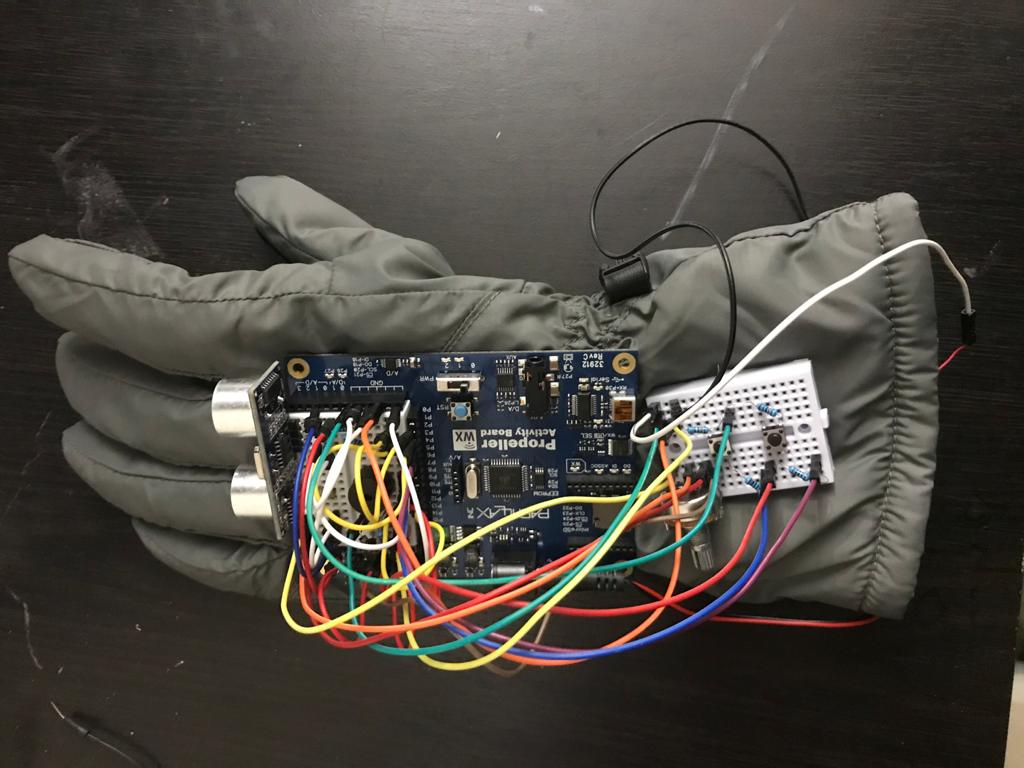
\includegraphics[width=\textwidth]{Propeller/Glove_Photo.jpeg}
        \caption{Photo of the product}
        \label{fig:glove}
\end{figure}

Ultrasonic Sensor, one of the most common distance sensing sensors out there, emits short high frequency (ultrasonic waves) at regular intervals, and the data received will have travelled up to the object, reflected back to the sensor. From the time taken to receive the data after transmission can help us find the distance of the object from the sensor. \\
A Vibration motor will be used to implement the physical actuation, for perception. The closer the object, higher the intensity of the vibration. The vibration motor used for this project has a voltage rating of 3V, so the precautions of capping the voltage output from the pin was done in the code. Theoretically, after a minimum threshold, a vibration motor should have a linear relation between the voltage input and the intensity of the vibration, however, the perceivable change in vibration intensity, for the vibration motor used in the model, ranged within 0.8V and 1.3V. For this reason, the operation of the vibration motor was restricted to this range. With a different Vibration Motor, this range will be different, however the maximum voltage output from a Parallax Propeller GPIO pin is 3.3V, so the maximum vibration is limited to 3.3V even though a certain vibration motor is capable of greater vibration, in this particular circuitry. \\
The range of the ultrasonic sensor HC-SR04 is 2-400cm, but for usability only a certain range with the threshold for maximum distance is taken. This threshold can be changed via a special mode called, \textbf{Distance Calibration Mode}. Similarly, the Maximum intensity of the vibration motor can also be changed by the user through \textbf{Vibration Calibration Mode}. The functionality of these \textbf{Calibration modes} is explained below.


\begin{enumerate}

    \item \large{\textbf{Distance Calibration Mode}}\\
    This feature was added in the light that blind people are aware of their personal space, and allows them to change the maximum distance observable.
    \begin{enumerate}
        \item \textbf{Activating the mode}\\ To activate the mode, the user will need to \textit{press the \underline{distance button} until it beeps}.\\
        \item \textbf{Calibration}\\ The user will need to stand a comfortable distance\footnote{The maximum distance cannot be greater than 300cm, due to the soft limits set} away from a wall, towards the end, this distance will be calibrated as the maximum distance observable. Once the mode is activated, the user will need to turn the potentiometer until a buzzer noise is heard, and then \textit{press the \underline{distance button} to set the distance}. \textit{To cancel} the calibration, at any point before pressing the calibration button, the user will need to \textit{press the \underline{vibration button}}. At the tone of the buzzer, the device is out of this mode. 
    \end{enumerate}
    
    \item \large{\textbf{Vibration Calibration Mode}}\\
    The user is given the option to change the intensity of Vibration felt while operating the device.
    \begin{enumerate}
        \item \textbf{Activating the mode}\\ To activate the mode, the user will need to \textit{press the \underline{vibration button} until it beeps}.\\
        \item \textbf{Calibration}\\ Once the mode is activated, the user will need to turn the potentiometer proportionally the user can feel the intensity of vibration change\footnote{Depending on the Vibration Motor, it maximum vibration cannot be changed past a point, so for usability, it is suggested to use it at less than the maximum perceivable vibration}; at the desired intensity, \textit{the \underline{vibration button} needs to be pressed to set} maximum intensity of vibration. \textit{To cancel} the configuration, at any point before pressing the vibration configuration button, the user will need to \textit{press the \underline{distance button}}. At the tone of the buzzer, the device is out of this mode.
    \end{enumerate}
    
    Exploiting EEPROM on the Parallax Propeller, the device does not require calibration every time it is powered down. The values set during both the calibration modes will be stored in the EEPROM and is reused all the time.
    
\end{enumerate}

\section{Circuit}
\begin{figure}[h!]
        \centering
        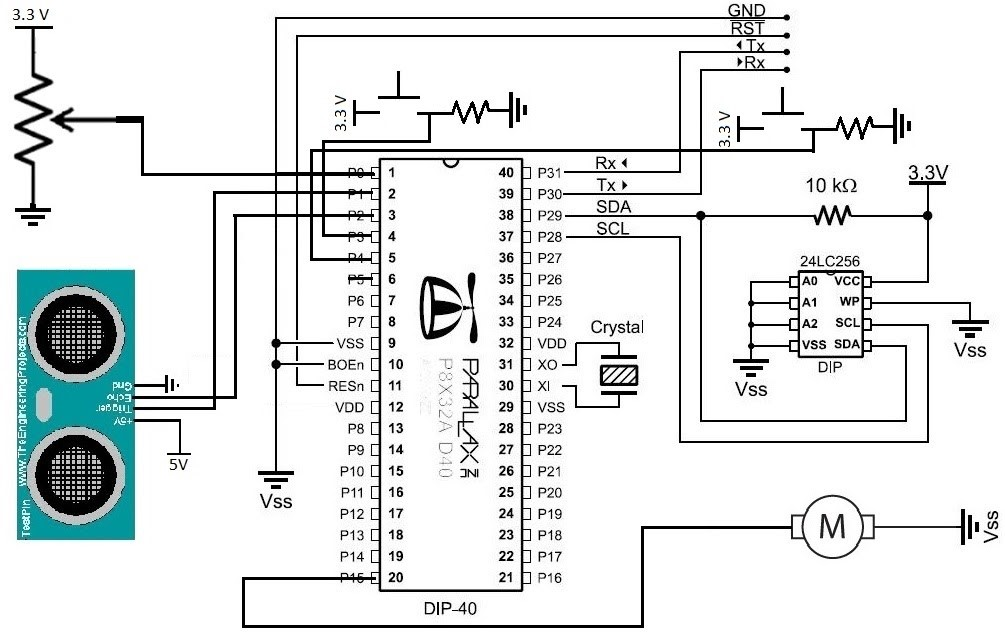
\includegraphics[width=\textwidth]{Propeller/circuit.jpg}
        \caption{Circuit Diagram}
        \label{fig:circuit}
\end{figure}

\section{Code}
\lstset{style=mystyle}

%Python code highlighting
\begin{lstlisting}[language=C]

#include "simpletools.h"                      // Include simple tools
#include "adcDCpropab.h"                      // Include adcDCpropab
i2c *eeBus;
#define Trig 1                                //Trigger for Ultrasonic sensor
#define Echo 2                                //Echo pin for Ultrasonic sensor
#define Pot  0                                //Potentiometer input 

#define VIB 9                                 //Vibration motor output
#define buzz 15                               //Buzzer output

#define cfg_but 3                             //Configure mode button (push button)
#define vib_but 4                             //Vibration configuation mode button (push button)

int ping(int TrigPin, int EchoPin);
int ping_cm(int TrigPin,int EchoPin);
int ping_inches(int TrigPin,int EchoPin);
int map(int var,int v_l1,int v_l2,int set_l1,int set_l2);
int vibration_intensity(int dist, int min_d,int  max_d);

void ultrasonicDistance(void *pauseTime);
void potentiometerReading(void *par);
void button_monitor();
void config_vibrate();
void configure();
void main_fun();
void button_m();
void firstTime();
static volatile int distance,potentiometer,pot_map_max_dist, pot_map_max_vib, max_dist, vib_max, config_button, vibrate_button;
static volatile int cog_ultra, cog_pot_met, cog_buttons, cog_vib, cog_cnfg, cog_main, cog_button;
static volatile float step_dist; 
unsigned int stack1[40+25];
unsigned int stack2[40+25];
unsigned int stack3[40+25];
unsigned int stack4[40+25];
unsigned int stack5[40+25];
unsigned int stack6[40+25];
unsigned int stack7[40+25];
static volatile int eeAddr = 0b1010000;
static volatile int memAddr_max_dist = 32768;
static volatile int memAddr_vib_max = 32773;
static volatile int memAddr_firstTime = 32778;
int check_val = 0;
int main()                                    // Main function
{
  eeBus = i2c_newbus(28,  29,   0);           // Set up I2C bus, get bus ID
  adc_init(21, 20, 19, 18);
  int pauseT = 60;
  i2c_in(eeBus,eeAddr,memAddr_firstTime,2,(char*) &check_val,4);
  if (check_val!=1)
  {
    firstTime();
  }
        
  i2c_in(eeBus, eeAddr, memAddr_max_dist,2,(char*) &max_dist,4);
  i2c_in(eeBus, eeAddr, memAddr_vib_max,2,(char*) &vib_max,4);

  cog_ultra = cogstart(&ultrasonicDistance, (void*)pauseT, stack1, sizeof(stack1));
  cog_pot_met = cogstart(&potentiometerReading, NULL, stack2, sizeof(stack2));
  cog_buttons = cogstart(&button_monitor, NULL, stack3, sizeof(stack3));  
  cog_main = cogstart(&main_fun, NULL, stack6, sizeof(stack6));

  while(1)                                    // Loop repeats indefinitely
  {
    putChar(HOME);                            // Cursor -> top-left "home"  
    print("potentiometer value = %d%c\n",potentiometer,CLREOL);
    print("distance measured = %d%c\n",distance,CLREOL);
    print("max dist set= %d%c\n",max_dist,CLREOL);
    print("max vib set= %d%c\n",vib_max,CLREOL);
    print("Distance Button = %d%c\n",config_button,CLREOL);
    print("Vibrate Button = %d%c\n", vibrate_button,CLREOL);
    print("Vibration = %d%c\n", map(distance, 2, max_dist,vib_max,67),CLREOL);
    pause(100);                               // Wait 1/10 s
  }  
}

void firstTime()
{
  int val =50;
  i2c_out(eeBus,eeAddr,memAddr_max_dist,2,(char*) &val,4);
  while(i2c_busy(eeBus,eeAddr));
  
  val = 150;
  i2c_out(eeBus,eeAddr,memAddr_vib_max,2,(char*) &val,4);
  while(i2c_busy(eeBus,eeAddr));
  
  val = 1;
  i2c_out(eeBus,eeAddr,memAddr_firstTime,2,(char*) &val,4);
  while(i2c_busy(eeBus,eeAddr));
}  

void main_fun(){
  while(1){
    if(distance <= max_dist){
      dac_ctr(VIB, 0, map(distance, 2, max_dist,vib_max,67));
    }
    else{
      dac_ctr(VIB, 0, 0);      
    }
  }          
}  



void ultrasonicDistance(void *pauseTime)
{
  int pauseT = (int)pauseTime;
  while(1)
  {
    distance = ping_cm(Trig,Echo);
    pause(pauseT);
  }    
}   

int ping(int TrigPin,int EchoPin)
{
  low(TrigPin);
  pulse_out(TrigPin, 10);
  return pulse_in(EchoPin, 1);
}

int ping_cm(int TrigPin,int EchoPin)
{
  long tEcho = ping(TrigPin,EchoPin);
  int cmDist = tEcho / 58.0;
  return cmDist;
}





int map(int var, int v_l1, int v_l2, int set_l1, int set_l2)
{
  float y;
  float a = 1.0* (set_l1 - set_l2)/(v_l1 - v_l2);
  float b = 1.0* (set_l1 - a*v_l1);
  y = a* var + b;
  return (int)y;
}  
int vibration_intensity(int dist, int min_d,int  max_d)
{
  step_dist = (max_d - min_d)/3.0;
  int  intensity = 80;
  if (dist*1.0 <= min_d*1.0+step_dist)
  {
    intensity = 150;
  }
  if ( dist*1.0 <= min_d*1.0+2.0*step_dist && dist*1.0 > min_d*1.0+step_dist)
  {
    intensity = 77;
  }        
    
  if (dist*1.0 <= max_d && dist*1.0 > min_d*1.0+2.0*step_dist)
  {
    intensity = 68;
  }  
  return intensity; 
  
}
  

void potentiometerReading(void *par)
{
  while(1)                                    // Loop repeats indefinitely
  {
    potentiometer = adc_in(Pot);
    pot_map_max_dist = map(potentiometer, 0,2650 ,30 ,300);
    pot_map_max_vib = map(potentiometer, 0, 2650, 80, 230);
    pause(10); 
  }    
}



void configure(){
  
  cogstop(cog_main);
  dac_ctr(VIB, 0, 0);
  freqout(buzz, 500, 3000);
  int flag = 0;
  int i = 0;
  while(config_button == 1);
  int count = 0;
  while(1){
    if( (distance < pot_map_max_dist + 3) && (distance > pot_map_max_dist - 3))
    {
      flag = pot_map_max_dist;
      dac_ctr(VIB, 0, 75);
      freqout(buzz, 10, 5000);
    }
    else
    {
      dac_ctr(VIB, 0, 0);
    }      
    if(config_button == 1)
    {
      max_dist = flag;
      freqout(buzz, 500, 3000);
      i2c_out(eeBus,eeAddr,memAddr_max_dist,2,(char*)&max_dist,4);
      while(i2c_busy(eeBus,eeAddr));
      freqout(buzz, 500, 3000);
      break;
    }     
    if(vibrate_button == 1)
    {
      freqout(buzz, 500, 4000);
    }         
   }
     
  cog_main = cogstart(&main_fun, NULL, stack6, sizeof(stack6));
  cogstop(cog_cnfg);    
}  



void config_vibrate(){
  cogstop(cog_main);
  dac_ctr(VIB, 0, 0);
  freqout(buzz, 500, 3000);
  int flag = 0;
  int i = 0;
  while(vibrate_button == 1);
  int count = 0;
  while(1){
      
      
    dac_ctr(VIB, 0, pot_map_max_vib);

     
    if(vibrate_button == 1)
    {
      vib_max = pot_map_max_vib;
      freqout(buzz, 500, 3000);
      i2c_out(eeBus,eeAddr,memAddr_vib_max,2,(char*) &vib_max,4);
      while(i2c_busy(eeBus,eeAddr));
      freqout(buzz, 500, 3000);

      break;
    } 
    if(config_button == 1 ) {
      freqout(buzz, 500, 4000);
      break;
    }            
   }
     
  cog_main = cogstart(&main_fun, NULL, stack6, sizeof(stack6));
  cogstop(cog_cnfg);    
} 



void button_m(){
  while(1){
  config_button = input(cfg_but);
  vibrate_button = input(vib_but);
  }  
}  



void button_monitor(){
  cog_button = cogstart(&button_m, NULL, stack7, sizeof(stack7));
  
  while(1){
  if(config_button == 1){
    for(int i = 0; i <= 100; i++){
     pause(10);
     if(config_button != 1){
      break;
     }       
    }
    if(config_button==1){
      cog_cnfg = cogstart(&configure, NULL, stack4, sizeof(stack4));
    }    
  } 
   if(vibrate_button == 1){
    for(int i = 0; i <= 100; i++){
     pause(10);
     if(vibrate_button != 1){
      break;
     }       
    }
    if(vibrate_button==1){
      cog_vib = cogstart(&config_vibrate, NULL, stack5, sizeof(stack5));
    }    
  } 
 
  }      
}
\end{lstlisting}

\section{Budget}
The Budget is clearly summarized in the table(\ref{tab:BOM}).

\begin{table}[h]
    \centering
    \begin{tabular}{|c|p{8cm}|l|}    \hline
    \textbf{Label} \#      &\textbf{Components}                     &\textbf{Cost}      \\\hline \hline
        1       &Parallax Propeller Activity Board                  &\$ 79.0            \\ \hline
        2       &Ultrasonic Sensor [HC-SR04]                        &\$ 4.20            \\ \hline
        3       &Vibration Motors [A00000117]                       &\$ 12.99           \\ \hline
        4       &Piezo Buzzer [A14121600UX0159]                     &\$ 2.19            \\ \hline
        5       &Potentiometer, push button, and other components   &\$ 10.00           \\ \hline \hline
                &Total                                              &\$ 107.28          \\ \hline
    \end{tabular}
    \caption{Bill of Materials}
    \label{tab:BOM}
    
\end{table}

\section{Conclusion and Future Work}
During this project, the cog functionality of the Propeller was explored to a great extent by utilizing seven cogs to perform the said task. Using I$^2$C protocol, the data from the RAM was stored in the EEPROM on the Propeller to remember the personalized calibration settings. Several hardware limitations like the perceivable vibration for a range of voltage input was discovered first hand, and precautions to work around them. The framework to replace the vibration motor on the device is already set, in the future iterations, a vibration motor with a more diverse range can be used to better perceive the distances, and potentially increase the comfortable distance range.  

\clearpage
\end{document}